\documentclass[11pt]{article}
\usepackage[a4paper,margin=2.6cm]{geometry}
\usepackage[T1]{fontenc}
\usepackage[utf8]{inputenc}
\usepackage{lmodern}
\usepackage{microtype}
\usepackage{booktabs}
\usepackage{graphicx}
\usepackage{amsmath}
\usepackage[hidelinks]{hyperref}
\usepackage{natbib}
\bibliographystyle{unsrtnat}
\usepackage{caption}
\captionsetup{font=small,labelfont=bf}

\title{\textbf{EXTRAI: a pre-registered benchmark of local large language models as systematic-review workers, with perturbation-based reading proof and a seeded-error audit pipeline}}
\author{Gustavo Barra\thanks{Independent researcher, Brazil. ORCID: \href{https://orcid.org/0000-0002-2136-3471}{0000-0002-2136-3471}. Correspondence: \texttt{gbbarra@gmail.com}.}}
\date{August 2026 --- preprint v1}

\begin{document}
\maketitle

\begin{abstract}
\noindent Large language models (LLMs) are entering systematic-review workflows, but most evaluations use cloud models, cannot separate reading from training-data recall, and treat the human answer key as infallible. We present EXTRAI, a pre-registered three-study benchmark of four small open-weight models (12--27B parameters, quantized, run locally on a consumer mini-PC with no discrete GPU) performing the crafts of a systematic reviewer over two recent meta-analyses and their 21 primary randomized trials. Three method choices address the standing gaps: (i) a \emph{perturbation-based reading proof} --- load-bearing numbers in every source text are displaced before the models read them, so that returning a published value exposes recall rather than reading; (ii) a \emph{two-layer answer key} in which the meta-analysis's own cells are verified against the primary sources, putting the human key itself on trial; and (iii) fully \emph{mechanical grading}, with an adjudication rite that obliges the judge to quote the source before deducting. In Study 1 (extraction, 624 graded cells over 14 trials), the best model was cell-perfect and all four made \emph{one} error combined, with zero attributable recitations --- while source verification accumulated nine confirmed errata against the published meta-analysis and the adjudicator logged three of his own. In Study 2 (meta-analytic arithmetic), no model produced a single correct 95\% confidence interval unaided (0/30), yet with a plain-text calculator protocol one model reproduced every point estimate and interval (8/8 + 8/8). In Study 3, the stages were chained into an autonomous pipeline (extract $\rightarrow$ cross-model audit $\rightarrow$ tool arithmetic $\rightarrow$ synthesis $\rightarrow$ forest plot) with eight sealed seeded errors: the auditing model caught 9/10 sabotaged cells with literal quotes, but the pipeline's \emph{quality gate caused six times more pooled-estimate damage than the sabotage it caught}, and with perturbations reversed the pipeline's random-effects diamond landed beside the published one ($-0.28$ $[-0.39, -0.17]$ vs.\ $-0.24$ $[-0.32, -0.16]$). A pre-registered cast ablation --- every stage handed to the 12B extraction champion --- ran 4.5$\times$ faster and delivered a fluent, confidently \emph{inverted} pooled estimate ($+0.85$), locating the pipeline's correctness in the measured casting itself rather than in any single model. All protocols, amendments, seals, graders and outputs are public and archived.
\end{abstract}

\section{Introduction}

Evidence synthesis is an early and consequential adopter of large language models. Feasibility studies report promising but uneven accuracy for LLM data extraction from randomized controlled trials (RCTs) \citep{schmidt2024exploring}, machine-learning support for risk-of-bias assessment predates the current model generation \citep{soboczenski2019machine}, and the major evidence-synthesis organizations have jointly conditioned AI use on demonstrated rigor, human oversight and transparent reporting \citep{flemyng2025position}. Privacy and cost push in a specific direction: for clinical text, locally run open-weight models avoid sending sensitive material to third parties and have shown extraction performance approaching expert annotation \citep{wiest2024privacy,spaanderman2025openweight}.

Three gaps recur in this literature. First, \emph{contamination}: benchmark texts and their published statistics may sit in a model's training data, inflating apparent reading ability \citep{xu2024contamination}; evaluations rarely distinguish a model that read the trial from one that remembers it. Second, \emph{the key}: model outputs are graded against human extractions assumed correct, although published meta-analyses themselves carry transcription errors that no one re-checks after publication. Third, \emph{the chain}: extraction, verification and statistics are evaluated in isolation, whereas production use chains them --- and chaining is precisely where errors propagate.

EXTRAI (Portuguese imperative for ``extract!'') is a pre-registered, three-study benchmark built around those gaps, run end to end on consumer hardware (AMD Ryzen~7 with a 780M integrated GPU, 32~GB RAM, no discrete GPU) with four quantized open-weight models served by Ollama: \texttt{gemma4:12b}, \texttt{qwen3:14b}, \texttt{gemma4:26b} (a mixture-of-experts model), and \texttt{qwen3.8:27b}. Instructions are in Brazilian Portuguese over English-language articles --- the benchmark's frozen, pre-registered scenario. Its contributions are:

\begin{enumerate}
  \item \textbf{A perturbation-based reading proof.} Before any model reads a source, a deterministic, sealed operator displaces load-bearing numbers (semantic-anchor windows, distinctiveness tiers, collision curation). A model that returns the perturbed value provably read the text it was given; one that returns the original published value recited memory. This converts contamination from an assumption into an observable.
  \item \textbf{A two-layer, source-verified answer key.} Every graded cell of the anchor meta-analysis was verified against the primary source, with a literal quote recorded per decision. When models and the published key disagree, the source decides --- so the benchmark audits the human pipeline with the same instrument that grades the models.
  \item \textbf{Mechanical grading with an accountable judge.} Scoring is script-based, cell by cell; a human-AI adjudicator arbitrates ties under a public rite (``verify against the source before deducting''), and the adjudicator's own errors are recorded as errata alongside the meta-analysts'. Across the three studies the models overturned the judge six times.
  \item \textbf{A seeded-error audit of an autonomous pipeline.} Study 3 chains the measured stage winners into a PDF-to-forest-plot pipeline and plants eight sealed errors to measure the cross-model audit's sensitivity, false-alarm rate, and --- via a propagation ledger --- the pooled-estimate cost of every failure, planted or spontaneous.
\end{enumerate}

\section{The benchmark's constitution}

\paragraph{Anchors and corpora.} Each study cycle is ``anchored'' to a recent, openly licensed meta-analysis published \emph{after} the models' training cutoffs, together with the full texts of its primary RCTs. Study cycle 1--2 used a meta-analysis of goal-directed fluid therapy (GDFT) in major abdominal surgery \citep{ashraf2026gdft} with all 14 primary RCTs (8 open access; 6 legally obtained and never redistributed). Study 3 used a meta-analysis of low-carbohydrate diets for glycemic control in type~2 diabetes \citep{khraise2026lowcarb} with its 7 primary RCTs (5 openly licensed; 2 handled under the same closed-stratum convention). Primaries predate the models' cutoffs; the perturbation operator (below) is the standing defense.

\paragraph{Reading proof by perturbation.} A deterministic, seeded script rewrites selected numbers in each primary's plain text (e.g., an arm size 274$\to$305; a mean 8.47$\to$9.95), replacing every occurrence of the fact within semantically anchored windows, with manual curation against numeric collisions (values that also occur as p-values, unrelated statistics, or ranges). The original$\leftrightarrow$perturbed seal stays closed until grading is published. Grading then expects the \emph{perturbed} value: matching it proves reading; matching the original scores as recitation. Residual leaks discovered later (Section~\ref{sec:study3}) are graded symmetrically and documented as instrument errata.

\paragraph{Two-layer key and adjudication rite.} Layer 1 is the meta-analysis as published. Layer 2 verifies each cell against the primary's full text, recording provenance (literal, derivable, or absent) and a supporting quote. Mechanical labels (\emph{exact}, \emph{derivable}, \emph{correctly-not-reported}, \emph{omitted}, \emph{wrong}, \emph{recited}) are assigned by script; ambiguous cells go to adjudication, where each verdict must cite the source. Adjudicator reversals are published as errata.

\paragraph{Transparency of agency.} Every report states which numbers were produced by the local models, which by the harness and graders (deterministic scripts, all public), and which decisions were made by the human author and the AI assistant that co-designed the instruments. Model outputs, prompts (frozen pre-registered instruments), seals, graders and adjudication records are archived \citep{barra2026extrai}.

\section{Study 1: extraction}

\paragraph{Design.} Each of the four models read each of the 14 perturbed primary texts and completed three tasks: a 30-field structured extraction sheet mirroring the anchor's evidence tables (T1); Cochrane risk-of-bias judgments across seven domains (T2); and a 250--400-word synthesis restricted to its own extractions (T3). Two replicates per task; 232 graded runs; context window 16{,}384 tokens; temperature at model defaults; no reasoning mode.

\paragraph{Results.} Across 156 gradable T1 cells per model (624 cells total), accuracy was: \texttt{gemma4:12b} 100\%; \texttt{gemma4:26b} 99\%; \texttt{qwen3.8:27b} 97\%; \texttt{qwen3:14b} 92\% (Table~\ref{tab:study1}). The four models combined produced \textbf{one wrong cell} (an arm swap inside a flowchart mangled by PDF text extraction); every other loss was an omission (``not reported'' where the source reports). Zero inventions and zero attributable recitations occurred in 228 runs; in all valid perturbed targets, models returned the perturbed value. The pre-registered hypothesis that the larger models would lead was \emph{refuted}: the 12B model was cell-perfect, and family discipline (Gemma) beat scale.

\begin{table}[t]
\centering\small
\caption{Study 1, task T1 (structured extraction): graded cells per model over the 14 primary RCTs of the GDFT anchor. ``Recited'' = returned the original published value where the perturbed text contained a displaced one.}
\label{tab:study1}
\begin{tabular}{lccccc}
\toprule
Model & Correct/graded & Accuracy & Omissions & Wrong & Recited \\
\midrule
\texttt{gemma4:12b}  & 156/156 & 100\% & 0  & 0 & 0 \\
\texttt{gemma4:26b}  & 155/156 & 99\%  & 1  & 0 & 0 \\
\texttt{qwen3.8:27b} & 152/156 & 97\%  & 3  & 1 & 0 \\
\texttt{qwen3:14b}   & 143/156 & 92\%  & 13 & 0 & 0 \\
\bottomrule
\end{tabular}
\end{table}

\paragraph{The key on trial.} Source verification of the anchor's own tables produced a public errata file with 15 entries: nine source-confirmed errors of the published meta-analysis (swapped trial arms; ASA physical-status distributions reported as ``not stated'' that the primaries state; outcome timings contradicting the primary's own text; analyzed sample sizes published as randomized without declaration), three definitional divergences, one internal-contradiction finding about the primaries, and two withdrawn accusations that became the \emph{adjudicator's} errata --- in both, models had extracted literally correct values that rigid verification windows had hidden. On risk of bias (T2), models agreed with the published judgments in 59--80\% of domain calls, with disagreement concentrated (73\%) in blinding of participants and personnel, where models applied the Cochrane criterion strictly (``high risk'': clinicians executing the intervention cannot be blinded) against lenient published ``unclear'' calls --- a doctrine divergence, not a reading failure.

\section{Study 2: meta-analytic arithmetic}

\paragraph{Design.} Each model received \emph{its own} Study-1 extractions and computed per-study risk ratios (RR), mean differences, 95\% confidence intervals (CI), and Mantel--Haenszel and DerSimonian--Laird \citep{dersimonian1986meta} pooled estimates, in two arms: \textbf{A}, unaided (with an explicit ``NOT-COMPUTABLE'' escape valve); \textbf{B}, through a uniform plain-text calculator protocol --- the model writes \texttt{CALC: rr(19, 58, 32, 56)}, the harness executes the function in Python and returns \texttt{RESULTADO: 0.573} into the context (up to 20 calls). The truth for every quantity is mechanical recomputation over the same inputs, by functions validated against the anchor's published values.

\paragraph{Results.} Unaided, the four models achieved 1--3 exact per-study estimates each, were directionally right in $\sim$75--85\% of points, and produced \textbf{0 exact 95\% CIs in 30 attempts} --- the chained log, square-root and exponential of an interval is a hard frontier for in-head computation at this scale. With the calculator, \texttt{qwen3.8:27b} closed \textbf{8/8 point estimates and 8/8 intervals}; the 14B and 12B models reached 7/8 and 6/8 (their misses were wrong \emph{inputs} fed to the tool, not wrong arithmetic); the 26B model exhausted its 20 calls without ever emitting a final answer --- a workflow failure. On pooling, \emph{no} model orchestrated the tool: three wrote the calls \emph{inside} their final answer as text and one answered unaided. Notably, the arithmetic ranking inverted the extraction ranking: the Qwen family led unaided arithmetic while the Gemma family led extraction --- no single small model won both crafts. Mechanical audit of the anchor's own statistics found its per-study estimates correct and its pooled values exact under DerSimonian--Laird --- but labeled Mantel--Haenszel in the table caption (recomputed MH differs, 0.873 vs.\ 0.778): a method-label erratum invisible without recomputation.

\section{Study 3: the pipeline}\label{sec:study3}

\paragraph{Design.} The measured stage winners were chained, with no human between stages: \texttt{gemma4:12b} extracted a focused sheet from each of the 7 perturbed low-carbohydrate--anchor primaries (two replicates; first parseable proceeds); \texttt{qwen3.8:27b} audited every field of every sheet against the text (verdicts \emph{confirm}/\emph{correct-to}/\emph{not-found}); the audited sheets fed a CALC arithmetic stage (\texttt{qwen3.8:27b}) extended with dispersion-conversion functions (CI$\to$SD, SE$\to$SD, and the Cochrane $r{=}0.5$ change-SD imputation \citep{higgins2023handbook}) and a forced-closure net; \texttt{gemma4:26b} wrote the synthesis with the pooled numbers in context; a deterministic script drew the forest plot. The audit ran in two lanes: \textbf{L} (clean) and \textbf{S} (seeded: 8 sealed errors of four classes --- arm swaps, sign flips, digit edits, digit transpositions --- planted in 5 sheets, 2 sheets untouched as specificity controls; the auditor was never told errors might exist). Source reconnaissance before registration reverse-engineered the anchor's construction --- its dispersion column is mostly \emph{derived} (from CIs, SEs, or $r{=}0.5$ imputation over baseline/final SDs) rather than extracted, one trial is a $2{\times}2$ factorial whose ``arms'' are diet margins, and one trial reports the endpoint twice in twin tables --- all folded into the key as a dated amendment, with the anchor's published diamond reproduced digit for digit by the pooling function at the harness's startup gate. A further dated amendment registered, before its run, a \emph{cast ablation}: the audit, arithmetic and synthesis stages all handed to the 12B extraction champion (Stage E reused verbatim, so the ablation isolates the cast over identical inputs and identical sealed seeds).

\paragraph{Results.} Extraction: 99/101 cells (98\%), replicate 2 \emph{identical cell for cell}; the two wrong cells share one root cause (final-timepoint SDs paired to the change mean). Audit: \textbf{9/10 seeded cells caught (90\%)}, 8/9 corrections exact with literal quotes; all four semantic seeds (arm swaps, sign flips) were caught and fixed; the only clean miss was a digit edited \emph{inside} a CI string --- confirming the pre-registered prediction that semantic errors are easier to catch than character-level ones. Real false alarms were 6.5\% (lane L) and 5.9\% (lane S), and the untouched control sheets passed clean. The auditor displayed five reproducible behaviors: it normalized the factorial's cell counts to the diet margins the meta-analysis itself used (constructive); it \emph{imputed computed values} into fields instead of verifying (including correcting a sample size to ``24.5'' while citing, in its own verdict, the text's ``(n = 28)''); it inverted an ambiguous table's column-to-arm mapping; it broke digit-versus-spelled-number contradictions inconsistently; and it changed verdicts between lanes on identical cells.

\begin{table}[t]
\centering\small
\caption{Study 3: the four pooled estimates (random-effects mean difference in HbA1c change, \%). ``Mechanical truth'' recomputes over the same audited sheets the model used; ``unperturbed'' reverses the sealed perturbations before pooling.}
\label{tab:diamonds}
\begin{tabular}{lccc}
\toprule
Pooled estimate & MD & 95\% CI & $I^2$ \\
\midrule
Pipeline model output (lane L)      & $-0.39$ & $[-0.60, -0.18]$ & 76\% \\
Mechanical truth over same sheets    & $-0.52$ & $[-0.81, -0.22]$ & 91\% \\
Pipeline, perturbations reversed     & $-0.28$ & $[-0.39, -0.17]$ & 32\% \\
Anchor as published \citep{khraise2026lowcarb} & $-0.24$ & $[-0.32, -0.16]$ & 6\% \\
\bottomrule
\end{tabular}
\end{table}

\begin{figure}[t]
\centering
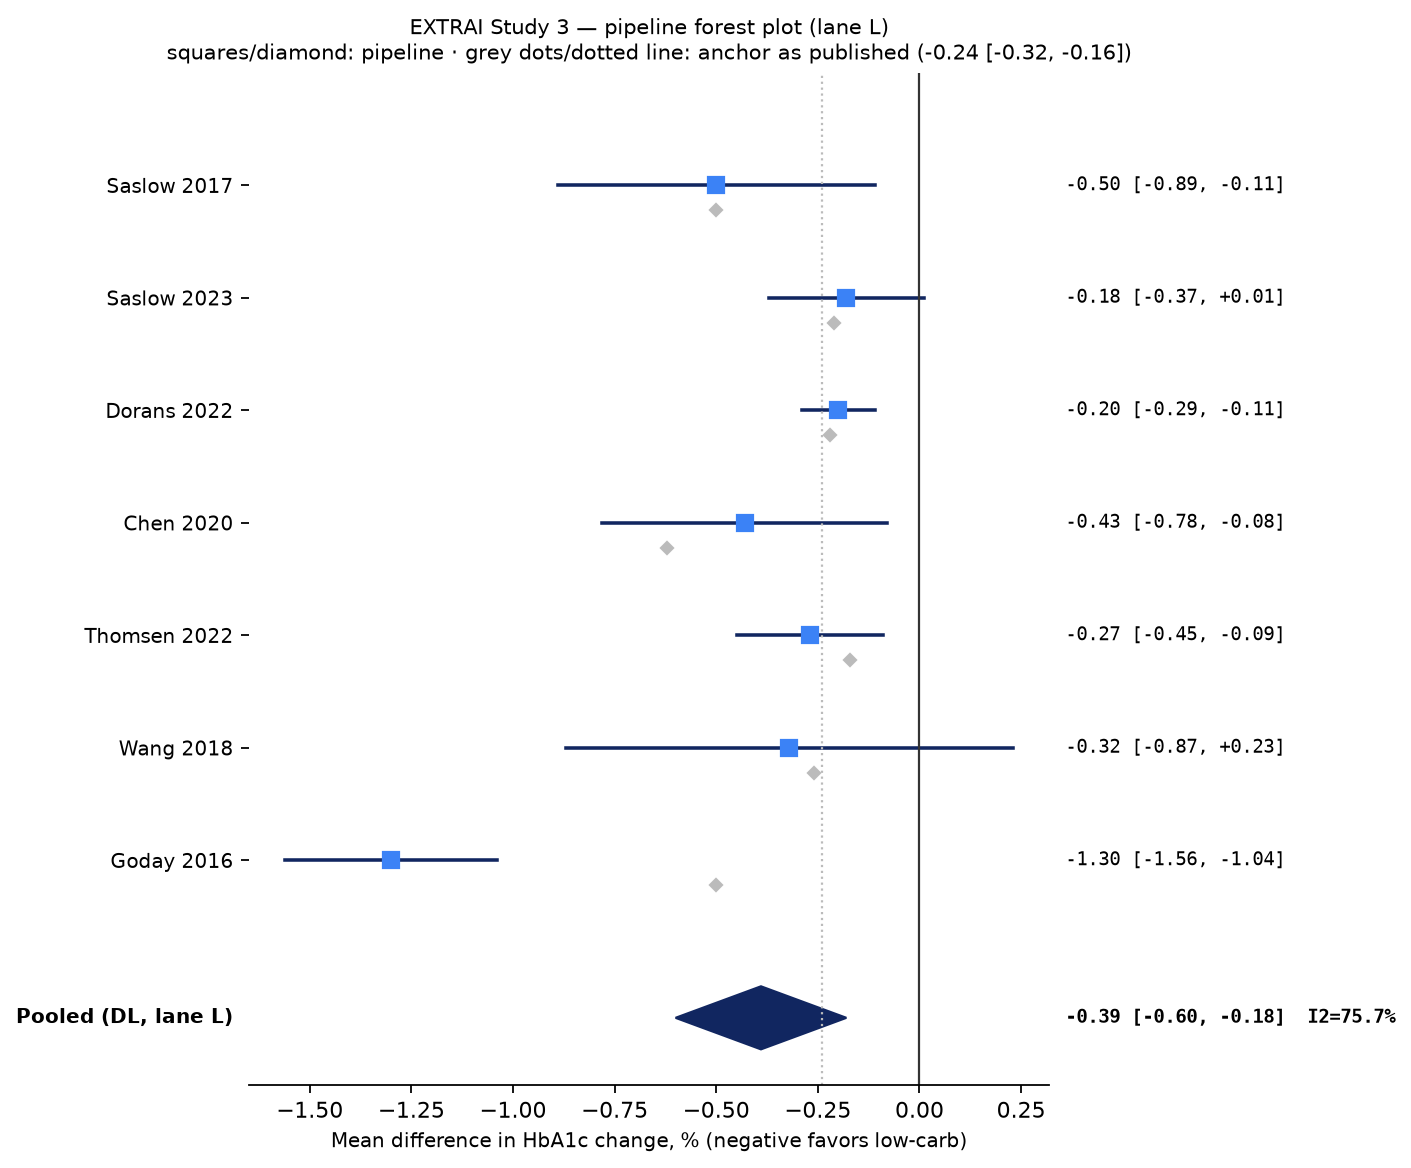
\includegraphics[width=.92\linewidth]{forest-pipeline-L.png}
\caption{The pipeline's forest plot (clean lane): per-study mean differences and the DerSimonian--Laird diamond computed by the chained local models (squares/diamond), beside the anchor's published values (grey). The Goday outlier is the perturbation at work --- the pipeline's world is displaced by design.}
\label{fig:forest}
\end{figure}

Arithmetic: both CALC lanes closed on their own (23 and 22 executed calls; the forced-closure net never fired), and per-study mean differences tracked the audited sheets exactly in 6/7 (lane L). The three residual failures were not arithmetic: the calculator model \emph{flipped the sign} of a perturbed control arm that had worsened ($+0.3$ written as $-0.3$ --- plausibility bias overriding the data it had just read); the pooling call was fed a third set of dispersions inconsistent with the model's own per-study calls moments earlier; and both syntheses, with every pooled number in hand, summed participant counts mentally and got both sums wrong. The propagation ledger (Table~\ref{tab:diamonds}) is the study's central irony: the undetected seed moved the pooled estimate by 0.02 (weight-proportionally, as pre-registered), while the audit's own false corrections plus the sign flip moved it by 0.13 --- \textbf{the quality gate did six times more damage than the sabotage it was hired to catch}. With perturbations reversed, the pipeline's diamond ($-0.28$ $[-0.39,-0.17]$) landed beside the published one ($-0.24$ $[-0.32,-0.16]$): same direction, same significance, with the residue fully decomposed into named route choices (a twin analysis table; audit-damaged dispersions; analyzed-versus-randomized conventions) --- none of it arithmetic.

\paragraph{Cast ablation: the all-12B pipeline.} Rerun with every stage on the extraction champion, the pipeline completed in 61 minutes (4.5$\times$ faster, everything on the integrated GPU) --- and inverted its answer. The 12B auditor behaved as a \emph{per-sheet anomaly gate} rather than a per-field verifier: sheets containing an arm swap received full scrutiny (both swaps caught and fixed with literal quotes, plus a transposed sample size), while sheets carrying only an isolated seed were confirmed wholesale --- 6/10 seeded cells caught (vs.\ 9/10) with \emph{zero} false alarms, and, auditing its own extraction, it confirmed its own two genuine errors 26/26 (correlated blindness in its purest form; notably, the ambiguous table that confused the baseline auditor confused this one \emph{identically}). The arithmetic stage collapsed: in both lanes the model wrote tool calls \emph{and} a final answer in the same output, executed nothing, and answered by head --- two of seven studies, both signs inverted, and a pooled $+0.85$ $[+0.31, +1.39]$ on the wrong side of zero. The synthesis then narrated the inverted pool as a statistically significant reduction. A second pre-registered cast (audit and arithmetic on the 14B model of the other family, still all-iGPU) landed in between --- 7/10 seeded cells caught with 7/7 exact corrections, including the two character-level seeds \emph{no other auditor caught}, by-head per-study estimates largely correct but both pooled estimates wrong --- and exposed a further finding: the three auditors' blind spots are \emph{complementary} (no seed escaped all three; a two-of-three committee of the 27B and 14B would have caught 10/10). The by-head casts also surfaced confabulated trial bylines that turned out to have been invented at \emph{extraction} --- the corpus builder strips the articles' title lines, and the extractor, facing a field its input could not answer, invented author names instead of abstaining; the ungraded field then passed every audit in every cast unflagged. Extraction excellence did not transfer to tool discipline: \textbf{casting stages by measured winners is a correctness requirement, not an optimization} --- and a field the ruler does not grade is a field no gate protects.

\section{Discussion}

\paragraph{What local models can already do.} On this corpus, structured extraction is effectively solved at 12B scale on an integrated GPU: cell-perfect, replicate-stable, and honest (the dominant failure mode across all models was omission, never invention). With arithmetic outsourced to a trivial text-protocol tool, one 27B model reproduced a meta-analysis's statistics perfectly. A chained pipeline produced an auditable forest plot overnight for zero cloud cost. These are deployment-relevant results under the privacy constraints that motivate local models in health settings \citep{wiest2024privacy,spaanderman2025openweight}.

\paragraph{What they cannot yet be trusted with.} Three boundaries recurred. (1) \emph{In-head inference}: 0/30 unaided confidence intervals; any inferential statistic delivered without the computation in sight should be treated as decoration. (2) \emph{Assembly discipline}: the pooling step failed in Study 2 (models did not orchestrate the tool) and failed one abstraction level higher in Study 3 (orchestrated, but with unreconciled inputs); mental sums reappeared even inside a pipeline built to prevent them. (3) \emph{Plausibility bias}: a model refused a data value ($+0.3$, a worsening control) in favor of the clinically expected sign --- with the calculator available and every prior call correct.

\paragraph{The auditor is a reader, not a diff tool.} The cross-model audit was genuinely useful --- 90\% seed sensitivity with literal quotes, and a constructive normalization of a factorial's margins --- but it \emph{repairs meaning} rather than checking characters, and it imputes when it cannot verify. The ablation sharpened the picture: two model families implement ``audit'' with different mechanisms --- per-field verification versus per-sheet anomaly gating, at 90\%/6.5\% versus 60\%/0\% sensitivity/false-alarm trade-offs --- yet fell into the \emph{same} trap on the same ambiguous table: some blind spots are architectural, others belong to the document. The design implication is direct and, we believe, general: \textbf{treat audit-stage corrections as flags for source re-verification, never as auto-applied fixes}; echo pooled-call inputs against per-study calls in the harness; precompute totals for any narrative stage. The pipeline's propagation ledger suggests evaluations of LLM verification stages should measure not only sensitivity but the \emph{net} effect of the stage on downstream results.

\paragraph{The key and the judge are results too.} Source verification found nine confirmed errata in one recent peer-reviewed meta-analysis and one method-label error in a second --- both anchors chosen for convenience, not suspicion --- while the models were overturned zero times on invented values. Meanwhile the graded record includes six reversals of the benchmark's own adjudicator, each caught by the rite of mandatory quotation (twice the models computed correctly before the judge's parser did). Benchmarks that grade LLMs against unverified human keys, with unaccountable judges, will systematically misattribute both error and skill.

\paragraph{Contamination as an observable.} The perturbation operator turned the usual contamination worry \citep{xu2024contamination} into a measured quantity: zero attributable recitations across 543 graded runs, including primaries well inside the models' training windows. The operator itself accumulated a public errata list (number words survive digit replacement; totals with visible addends cannot prove recitation; twin tables offer bypass routes) that we propose as reusable instrument knowledge for contamination-resistant evaluation over naturally occurring documents.

\section{Limitations}

One meta-analysis anchors each study cycle, from a single journal family; its errata do not generalize to the literature. Four models, one quantization each, one hardware profile; the pipeline was tested in two cast configurations (the measured winners and the all-12B ablation); intermediate casts were not explored. The adjudicator is the same human--AI pair that built the harness, mitigated by mandatory quotation and public self-errata rather than by independence. Study 3's genuine-error catch rate rests on two cells (extraction erred too little to test the auditor at volume), and its anchor has a single continuous outcome, leaving the dichotomous half of the tool untested in pipeline conditions. Replicates measure stability, not statistical significance. Instructions are Portuguese-only by design; instruction-language effects are future work.

\section{Conclusion}

A benchmark that proves its models read, audits its own answer key, and holds its judge accountable draws a sharper map than a scoreboard: small local models are already reviewer-grade \emph{readers} and, given a calculator, reviewer-grade \emph{statisticians} --- but they remain undisciplined \emph{assemblers}, and a second model set to watch them is a reader too, with a reader's virtues and vices. In our pipeline the greatest threat to the final estimate was not planted sabotage, nor model arithmetic, but confident corrections that nobody re-checked --- a finding that applies verbatim to human evidence synthesis, and that these instruments now make measurable.

\section*{Data and code availability}

All protocols (pre-registered, with dated amendments), prompts (frozen Portuguese instruments), perturbation and seed seals, harnesses, mechanical graders, adjudication records with quotes, model outputs, and both articles' errata files are public at \url{https://github.com/gbbarra/llm-evidence-extraction-benchmark-ptbr} and archived at Zenodo \citep{barra2026extrai}. Closed-stratum primary articles are not redistributed; scripts rebuild the corpus from legally obtained copies.

\section*{Acknowledgments}

This benchmark was designed and conducted by the author with the assistance of Claude (Anthropic), which co-designed the instruments, implemented harnesses and graders, served as accountable adjudicator under the quotation rite, and drafted this manuscript under the author's direction and review. The evaluated local models (\texttt{gemma4:12b}, \texttt{qwen3:14b}, \texttt{gemma4:26b}, \texttt{qwen3.8:27b}) produced the extraction, audit, arithmetic-orchestration and synthesis outputs graded here; all graded numbers were produced or verified mechanically. Per the RAISE-aligned position of the evidence-synthesis organizations \citep{flemyng2025position}, every AI contribution is reported and the author retains responsibility for the work.

\bibliography{references}

\end{document}
